\chapter{广播和本地组播(IGMP 和 MLD)}

\minitoc
\section{引言}
第2章中我们提到有4种IP 地址:单播(unicast)、任播(anycast)、组播(multicast)
和广播(broadcast)。IPv4 可以使用所有这些地址,而IPv6可以使用除了最后一种形式的所
有其他形式的地址。在本章中,我们讨论广播和组播更多的细节,包括链路层地址如何有效
地用于从一台计算机向其他几台计算机发送组播或广播流量。我们也查看互联网组管理协议
(IGMP) \href{https://www.rfc-editor.org/rfc/rfc3376}{[RFC3376]}和 IPv6组播侦听发现(MLD)\href{https://www.rfc-editor.org/rfc/rfc3810}{[RFC3810]}协议,它们用来通知IPv4 和
IPv6 组播路由器子网中哪些组播地址在使用中。本章(或本书)中,我们没有涉及的一个主
题是在诸如全球互联网的广域网中,组播路由是如何实现的。目前,组播在企业和本地网络
中的使用超过在广域网中的使用。尽管我们在本章中讨论的这些协议是为了完全理解广域组
播,但是广域路由协议比较复杂,而且会使解释本地局域网的情况不必要地复杂化。对探索
这些问题感兴趣的读者可以参考[EGW02]。

广播和组播为应用程序提供了两种服务:数据分组交付至多个目的地,通过客户端请
求/发现服务器。

\begin{itemize}
    \item 交付至多个目的地。有许多应用程序将信息交付至多个收件方,例如,互动式会议、
    邮件或新闻分发至多个收件方。没有广播或组播,这些类型的服务往往倾向于使用现
    在的TCP(将一个单独的副本交付至每一个目的地,这是非常低效的)。
    \item 通过客户端请求服务器。使用广播或组播,应用程序可以向一个服务器发送一个请
    求,而不用知道任何特定服务器的IP 地址。当本地网络环境的信息了解得很少时,
    这种功能在配置过程中非常有用。例如,一台笔记本电脑可能需要使用 DHCP,获取
    它的初始IP地址,找到其最近的路由器(见第6章)。
\end{itemize}

虽然广播和组播都可以提供这些重要的功能,但是相对于广播来说,组播一般情况下是
更可取的,因为组播只涉及那些支持或使用特定服务或协议的系统,而广播却不是。因此,
一个广播请求会影响在广播范围内所有可以到达的主机,而组播只影响那些可能对该请求有
兴趣的主机。当我们探讨广播和组播的详细情况后,这些概念将变得更加清晰。现在,请记
住,在广播的更高开销和简单性以及组播的效率改善和更多的复杂性之间存在一种平衡。

广播自出现以来,就一直受到 IPv4 协议的支持,而随着\href{https://www.rfc-editor.org/rfc/rfc1112}{[RFC1112]}的出版,组播被添
加进来。IPv6 支持组播但不支持广播。一般来说,只有使用 UDP 传输协议(第10章)的用
户应用程序利用广播和组播,此时应用程序发送单个报文到多个收件方才是有意义的。TCP
是一个面向连接的协议,这意味着两台主机(由IP地址指定)和每台主机上的一个进程(由
端口号指定)之间的一个连接。TCP 可以使用单播和任播地址(回想一下,任播地址可以像
单播地址一样),但是不能使用广播或组播地址。


\begin{tcolorbox}
    广播和组播也被一些重要的系统进程使用,如路由协议、ARP、IPV6 中的
ND 等。虽然IP 组播支持曾经是 “插件”,要求用户给系统打补丁以使用它,但是
现代的操作系统默认地包括这种功能。组播是重要的,但在 IPv4 中是可选的功能,
而在IPV6中,因为ND 中使用它,所以是强制性的。ND 对单播通信来说是关键的
服务。
\end{tcolorbox}

\section{广播}
广播是指将报文发送到网络中的所有可能的接收者。在原理上,这是简单的:路由器简
单地将它接收到的任意报文副本转离(forward out)除报文到达的接口以外的每个接口。当
有多个主机连接到同一个本地局域网时,事情就稍微有点复杂了。在这种情况下,链路层的
特点可以使得广播在某种程度上更高效。

考虑在诸如以太网的网络上的一组主机,这种网络在链路层上支持广播。每个以太网帧
包含源和目的MAC地址(48位值)。通常情况下,每个IP 分组被指定到一个单一的主机,
所以使用单播寻址,目的地的唯一MAC地址使用ARP或IPv6 ND 来确定。当一个帧以这
种方式被发送到一个单播目的地时,任意两个主机之间的通信不会打扰网络上的任何其他主
机。对于交换以太网来说,这些都是在交换机和网桥中的站点缓存中发现的地址类型(见第
3章)。然而,有些时候,一个主机要向网络(或VLAN)上的每个其他主机发送一个帧一
这称广播 (broadcast)。在第4章中,与ARP一起,我们看到了这一点。

\subsection{使用广播地址}
在一个以太网或类似网络中,组播MAC地址中高位字节的低序位打开。以十六进制表
示,这看起来像01:00:00:00:00:00。我们可以认为以太网广播地址 ff:ff:ff:ff:ff:ff 是以太网组
播地址的一种特情况。从第2章中可以回忆到,在IPv4 中,每个子网都有一个本地定向
子网广播地址,它是通过将地址中的主机部分全部置1形成的,特殊地址 255.255.255.255
对应于本地网络(也称为“有限”)广播。

\subsubsection{例子}
在Linux 中,与每个接口相关的1Pv4 定向子网广播地址可以通过ifconfg命令查看或设

置。我们可以看到它显示如下:
\begin{verbatim}
Linux& ifconfig etho
ethO    Link encap: Ethernet    HWaddr 00:08:74:93:C8:3C
        inet addr:10.0.0.13     Bcast:10.0.0.127   Mask:255.255.255.128
        inet6 addr: 2001:5c0:9ae2:0:208:74ff:fe93:c83c/64
                Scope:global
        inet6 addr:fe80::208:74ff:fe93:c83c/64
                Scope:Link
        UP BROADCAST RUNNING MULTICAST MTU:1500

Metric:1

RX packets: 426469 errors:0 dropped:0 overruns:1 frame:0

TX packets: 779338 errors:0 dropped:0 overruns:0

carrier:0

collisions:298048 txgueuelen:1000

RX bytes:44414543 (42.3 MiB)

TX bytes:1094425223(1.0GiB)

Interrupt:19 Base

address:0xec0O
\end{verbatim}

这里,地址 10.0.0.127是设备 etho所连接的网络上使用的(定向子网)广播地址。它是
通过获取网络前缀(10.0.0.0/25),并将其与该地址的主机部分的32-25=7位的1相结合
来形成的:10.0.0.0OR 0.0.0.127=10.0.0.127。一个称ipcalc 的简单工具在某些系统上可
以用来执行世计算。

为了查看简单的广播是如何工作的,我们可以使用ping 程序向 ifconfig 命令输出中指明
的广播地址 10.0.0.127 发送一个ICMPv4 回显请求报文:

\begin{verbatim}
    
Linux# ping -b 10.0.0.127

WARNING: pinging broadcast

address

PING 10.0.0.127(10.0.0.127)56(84)bytes of data.

64 bytes from 10.0.0.6: icmp\_seq=1 tt1=64 time=1.05 ms

64 bytes from

10.0.0.113: icmp\_seq=1 tt1=64 time=1.55 ms

64 bytes from 10.0.0.120:icmp\_seq=1 tt1=64 time=3.09 ms

--- 10.0.0.127 ping statistics ---

1 packets transmitted,1 received,+2 duplicates,

0% packet loss,time 0ms
\end{verbatim}

我们在第8章中提到过,在这种类型的广播中,本地LAN(或 VLAN)上的所有主机都
受影响。在这里,我们收到了网络上的三个其他主机的回复,并且 ping 程序说明接收到了比
发送的请求数量更多的响应(DUP!指示)。为了查看正在使用的地址,我们使用Wireshark
来研究该活动(见图9-1)。

\begin{figure}[ht]
    \centering
	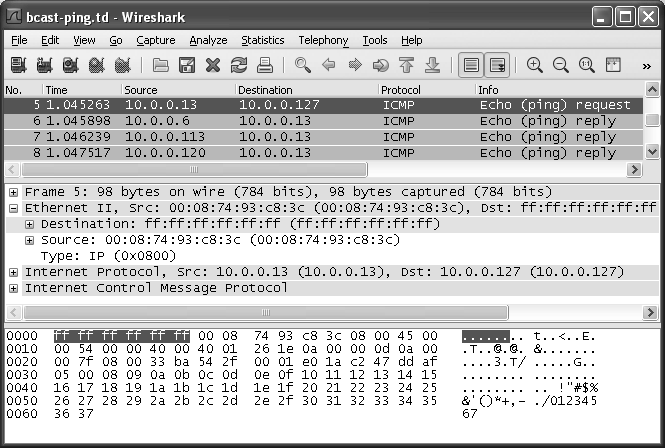
\includegraphics[width=0.7\textwidth]{imgs/9/9-1.png}
	\caption{发送到本地子网定向广播地址的ICMPv4 回显请求报文被封装在一个链路层广播帧中,并且该帧的目的地址全部为1}
\end{figure}

回显请求报文被发送到地址 10.0.0.127。IPv4 的实现通过咨询本地路由表中的信息和接
口配置信息,确定这是该定向子网的广播地址,并且它使用链路层广播地址ff:ff:ff:ff:ff:ff 发
送该数据报,因此不需要 ARP 请求来确定每个目的地的 MAC地址。事实上,在主机响应之
前,发送方并不知道哪个主机将响应。它只知道10.0.0.127是一个广播地址,因此当它发送
时,应该使用广播链路层目的地址。在IP 层和链路层的源地址全部是传统的单播地址;组
播地址只能作为目的地址。

在这个特定的例子中,请注意,每个生成的响应被定向到 10.0.0.13、原始发送方的单播
地址,并且每个响应包括响应方的IPv4地址:10.0.0.6,10.0.0.113 和 10.0.0.120。这是一个
原理更普遍的简单例子:广播寻址(和组播寻址,不久我们将看到)可以用来发现其他方面
未知的系统或服务。在这个例子中,传出的广播 ping 请求发现了三个主机,它们愿意响应广
播回显请求报文。

\subsection{发送广播数据报}
一般来说,使用广播的应用程序使用UDP协议(或ICMPv4协议),然后调用一组普
通API来发送流量。唯一例外的是,当调用API 时,一些操作系统会使用一个特殊的标志
(SO\_BROADCAST),以表示该应用程序确实打算发送广播数据报。例如,在Linux 中,当
试图发送广播 ping 时,没有使用-b 标志会引起下面的输出:

Linux8 ping

10.0.0.127

Do you want to ping broadcast? Then -b

之所以引起该错误,是因为只有在命令中提供-b 参数时,才能通过API 提供SO.
BROADCAST
标志。这有助于避免意外产生广播流量而造成暂时拥塞网络。

为了确定哪些接口用于广播,可以咨询 IPv4转发表(这里称为“路由表”)。以下是
Windows Vista 路由表的一个例子(更高版本的Windows 使用完全相同的格式),显示了接口
列表和广播相关的路由信息(为清楚起见,其他信息已被移除):

\begin{verbatim}

\end{verbatim}

输出的第一部分显示了7个不同的网络接口,它们可用于承载网络流量。第1个是虚拟
环回接口,下一个是 Wi-Fi无线接口,第3个是有线以太网接口(断开的),第4个是另一个
环回接口,随后的三个用作非标准站内自动隧道寻址协议(ISATAP)\href{https://www.rfc-editor.org/rfc/rfc5214}{[RFC5214]} \href{https://www.rfc-editor.org/rfc/rfc5579}{[RFC5579]}
的一部分。ISATAP 用于支持由 IPv4 网络隔断的IPv6 主机。

转移到路由表中,我们可以看到有7个项目能够用于确定广播流量应发送到的地址。第
一项是默认路由(掩码为 0.0.0.0),所以它匹配任意的目的地。如果有这样的设施启用了,
就可以被定向广播用于跨越本地网络。这种类型的定向广播移动到本地网络之外,通常由路
由器来禁用,以避免一些安全问题,如\href{https://www.rfc-editor.org/rfc/rfc2644}{[RFC2644]}所建议的。

接下来的三个条目分别是与IPv4地址10.0.0.57、127.0.0.1 和 169.254.57.240 相关的3个接
口的定向子网广播地址。最后两个是软件环回接口。这些条目说明Windows如何通过结合网
络前缀与全1主机位作为定向子网广播路由的目的地址,以及子网掩码/32 或 255.255.255.255。
Gateway 列 On-link,所以使用直接交付(见第5章)将流量交付至 Interface 列中指定的接口
上。在这些情况下,对于每个定向广播地址,至多有一个匹配,因此不会询问 Metric列。

最后三项是有限广播地址的路由条目,255.255.255.255。在某些时候,这个地址像组播
地址一样,因为它不直接与任意直接连在网络上的正在使用的地址相关联。因此,哪一个
接口应该用于发送去往有限广播地址的流量不是一目了然的。不幸的是,Host Requirements
RFC \href{https://www.rfc-editor.org/rfc/rfc1122}{[RFC1122]} 的3.3.6 节提供了很少的指导:

目标地址为有限广播地址的数据报是否应该从多宿主主机的所有接口发送,对
此已有讨论。此规范对该问题不持任何观点。

因此,到有限广播地址传出流量的处理方式是特定于操作系统的。大多数系统都选取一
个单一的具有广播功能的接口来发送这样的流量。Linux 和 FreeBSD按这种方式运行。事实
上FreeBSD将有限广播地址转换成一个“主”(第一次配置)接口的定向子网广播地址,虽然
应用程序可以使用IP\_ONESBCAST API 参数来禁用此行为。例如,Windows 在不同的版本
中表现不同。一直到 Windows 2000,有限广播都通过多个接口来转发。在 Windows XP 及稍
后版本中,默认的动作是通过一个单一的接口来发送。在这个例子中,对于这样的流量有多
个可能的匹配路由,所以使用了具有最低跃点数的条目(接口10.0.0.57)。

\section{组播}
为了减少在广播中涉及的开销,可以只向那些对它感兴趣的接收方发送流量。这被称为
组播(multicasting)。从根本上说,通过发送方指明接收方,或是通过接收方独立地指明它
们的兴趣,就可以完成这项工作。然后网络只负责向预期的/感兴趣的收件方来发送流量。
实现组播比广播更具挑战性,因为组播状态(multicast state)(信息)必须由主机和路由器来
保持,以说明哪些接收方对哪类流量有兴趣。在组播TCPAIP模型中,接收方通过指明组播
地址和可选源列表来表明它们对希望接收的流量的兴趣。这个信息作为主机和路由器中的软
状态(soft state)(见第4章)来维持,这意味着它必须定期更新或是超时删除。当这发生时,
组播流量的交付要么停止,要么恢复为广播。

广播的低效不仅体现在广域网中,此时它们是极其严重的,同时也体现在局域网和企业

网络中。在相同LAN或VLAN上可以到达的每个主机必须处理广播分组。IP 组播提供了一
个更有效的方式以执行相同类型的任务。如果正确地使用IP组播,只有那些在通信中参与
或感兴趣的主机需要处理相关的分组,流量只会被承载于它将被使用的链路上,并且只有任
意组播数据报的一个副本被承载于任意的这样的链路上。为了使组播工作,希望参与通信的
应用程序需要一种机制来发布其意愿的协议实现。然后主机软件可以安排接收与应用程序的
条件相匹配的分组。

IP组播在诸如以太网的链路层网络中,起初使用一种基于组寻址工作方式的设计。在
这种方法中,每个站点选择它愿意接收流量的组地址,而不考虑发送方。因对于发送方的
身份是不敏感的,所以这种方法有时也被称为任源组播(ASM)。由于IP 组播已经演化了,
另一种代替方式已经研究出来,它对于发送方的身份是敏感的,被称为特定源组播(SSM)
[RFC46071,它允许终端站点明确地包含或排除从一组特定发送方发送到一个组播组的流量。
SSM服务模型比 ASM更容易实现,这主要是因为在广域组播中,确定单个源的位置比确定
很多源的位置更容易。然而,在局部区域,支持ASM 或SSM的大部分机器是相同的,所以
我们把它们放在一起,并且只有当差异很重要时,才解释这些差异。下面我们开始研究在具
有组播功能的IEEE LAN技术中,IP组播流量是如何使用MAC层组播地址的。

\subsection{将IP 组播地址转换为 802 MAC/ 以太网地址}

在类似以太网的网络中,使用单播地址时,ARP(见第4章)通常根据目的地的IPv4地
址确定其 MAC地址。在IPv6中,ND起着类似的作用(见第8章)。当我们查看早期的广播
时,我们注意到,有一个众所周知的广播MAC地址,可以用于达到一个 LAN或VLAN上
的所有站点。当我们想要发送组播流量时,什么样的目的地 MAC地址应该放置于链路层帧
中呢?理想的情况下,我们不必使用协议报文来确定适当的 MAC地址,相反,可以只是简
单地将一个IP组播地址直接映射到一些对应的 MAC地址。了了解这是如何完成的,我们
会专注于IEEE 802 网络,特别是以太网和 Wi-Fi。这些网络代表了使用IP组播的最常见的
网络类型。首先,我们将讨论与IPv4 相关的映射如何进行,然后转移到在IPv6中使用的略
有不同的方法。

为了在链路层网络中有效地承载IP 组播,在IP 层和链路层帧的数据分组和地址之间
应该有一个一对一的映射。IANA 拥有IEEE组织唯一标识符(以下简称 OUI,或非正式
称为以太网地址前缀)00:00:5e。有了它,IANA 就被赋予权限去使用以01:00:5e开始的
组(组播)MAC地址以及以 01:00:5e 开始的单播地址。该前缀被用作以太网地址的高序24
位,这意味着此块包括范围在 00:00:5e:00:00:00到 00:00:5e:ff:ff:ff的单播地址,以及范围在
01:00:5e:00:00:00到 01:00:5e:ff:ff:ff 的组播地址。除了IANA 的其他组织也拥有地址块,但
只有IANA将其空间的一部分用于支持IP 组播。

IANA分配一半的组地址块用于识别 IEEE 802 LAN上的IPv4 组播流量。这意味着,对
应到IPv4组播的以太网地址范围为 01:00:5e:00:00:00 到 01:00:5e:7f:ff:ff。

\begin{tcolorbox}
    此处我们使用互联网标准位序来表示,即内存中位出现的顺序。这是大多数
    程序员和系统管理员处理的方式。IEEE 文档中使用位的传输顺序。
\end{tcolorbox}

IPV4 地址到它们对应的IEEE 802 形式的链路层地址的映射如图9-2所示。

图9-2 IPv4- 到IEEE 802 MAC组播地址的映射使用IPv4组播地址的低序23位作为以 01:00:5e 开始
的MAC地址的后缀。因为只使用了28个组地址位中的23位,32个组地址被映射到相同的MAC 层地址

回忆第2章,所有的IPv4 组播地址都被包含在从 224.0.0.0到239.255.255.255 的地址空
间中(以前称为D类地址空间)。所有这样的地址在高序位共享一个共同的4位序列1110。
因此,有32-4=28位可用来编码整个空间,即22=268 435 456 个组播 IPv4 地址(也称
为组ID)。对于 IPv4,IANA 的政策是分配一半的组地址用于支持IPv4 组播,这意味着所有
的268 435 456个组播组ID 需要被映射到只包含22=8388608个唯一条目的链路层地址空
间。因此,映射是非唯一的(nonunique)。即多个 IPv4组ID 被映射到相同MAC层组地址。
具体来说,22/22=2’=32个不同的IPv4组播组ID 被映射到每个组地址。例如,组播地址
224.128.64.32(十六进制 e0.80.40.20)和224.0.64.32(十六进制为€0.00.40.20)都被映射
到以太网地址 01:00:5e:00:40:20。

对于 IPv6,16位的OUI 十六进制前缀是 33:33。这意味着,IPv6地址的最后32位可以
用来形成链路层地址。因此,任何以相同的32位结束的地址映射到相同的MAC 地址(见
图9-3)。由于所有的IPv6组播地址以 ff开始,随后的8位用于标志和范围信息,这就留下
128-16=112 位用于表示2 个组。因此,MAC层地址的32位可用来编码这些组,可能
有多达2!2/232=280个组映射到相同的 MAC地址!

图9-3 IPv6到IEEE-802 MAC组播地址映射使用IPv6组播地址的低序32位作以33:33开始的
MAC地址的后缀。因为只使用了112个组播地址位中的32位,所以280个组映射到相同的
MAC层地址

\subsection{例子}
在前面的例子中,我们使用一个子网广播地址,以确定所有的本地子网中的主机,它

们将响应广播ICMPv4 回显请求报文。在这里,因为我们可以使用组播地址来确定提供特
定服务的主机,我们可以向那些响应组播 DNS(mDNS [CK11])地址224.0.0.251 的主机发送
ICMPv4 回显请求报文。

\begin{verbatim}
    
Linux& ping 224.0.0.251

PING 224.0.0.251(224.0.0.251)56(84)bytes of data.

64 bytes from 10.0.0.2:icmp\_seq=1 tt1=60 time=1.10 ms

from

10.0.0.11:icmp\_seq=1 tt1=60 time=1.60 ms (DUP!)

64 bytes from 10.0.0.120:icmp\_seg=1 tt1=64 time=2.59 ms (DUP!)

--- 224.0.0.251 ping statistics ---

1 packets

transmitted,1 received,+2 duplicates,

08 packet loss,time 0ms

rtt min/avg/max/mdev = 1.109/1.767/2.590/0.615 ms
\end{verbatim}

在这里,主机 10.0.0.2、10.0.0.11和10.0.0.120全部响应,表明它们订阅了mDNS组。

请注意,这些主机和我们使用广播地址10.0.0.127时响应的主机是不相同的。这并不奇怪
因为不是所有的主机都支持mDNS 协议。

注意

组播DNS(mDNS的)是一个服务,它旨在支持零配置(容易的系统和

设备配置)。mDNS已经由苹果系统支持,它作为Bonjour的一部分。微软已经

推出的一种替代协议也有类似的功能,被称为链路本地组播名称解析(LLMINR)

\href{https://www.rfc-editor.org/rfc/rfc4795}{[RFC4795]}。目前这两个协议都不是IETF 内的互联网标准,但现在,mDNS具有

比LLMNR 更长的历史。有关详细信息请参阅第11 章。

对于 IPv6,我们可以使用ICMPv6 回显请求报文执行相同的操作。

Linux8.ping6 -I etho ff02::fb

PING ff02::fb(ff02::fb) from fe80::208:74ff:fe93:c83c eth0:

56 data bytes

64 bytes

from

fe80::217:f2ff:fee7:6d91:icmp\_seg=1 tt1=64 time=2.76 ms

--- ff02::fb ping statistics

1 packets transmitted,1 received,0%

packet loss,time 0ms

rtt min/avg/max/mdev = 2.768/2.768/2.768/0.000 ms

请注意,在这种情况下,我们提供了传出接口作为ping6 程序的输人。这允许程序在

Windows XP 中选择合适的传出IPv6地址。在图9-4中我们可以看到,选择的地址是与设备
ethO 相关的本地链路地址。

\begin{figure}[ht]
    \centering
	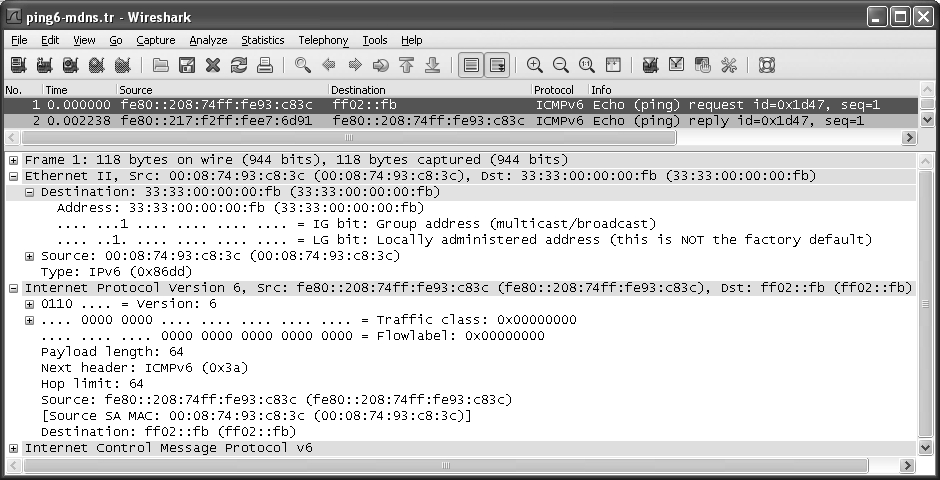
\includegraphics[width=1\textwidth]{imgs/9/9-4.png}
	\caption{ICMP 回显请求报文由与ethO网络接口相关的本地链路单播地址发送到组播地址ff02::fb。应答包含发送方的IPv6 本地链路IPv6地址}
\end{figure}

被识别为ICMPv6 回显请求/应答报文的数据分组中的标识符(Identifier)字段设置为
0x1d47,序列号(Sequence Number)字段设置1。在所有情况下,源IPv6地址是本地链
路的。请求的目的地址是组播地址 ff02::1b,它被映射到 MAC地址33:33:00:00:00:tb。回显
应答报文由响应方的本地链路单播地址 fe80::217:f2ff:fee7:6d91,直接发送到发送方的本地
链路单播地址 fe80:208:74 FF:fe93:c83c。需要注意的是,回显应答报文的发送方安排使用相
同范围内的源 IPv6地址(见在第5章中源地址选择的讨论,并比较图9-4和图5-16)。

\subsection{发送组播数据报}
当发送任意的IP数据分组时,必须决定使用哪个地址和接口。对于IPv6来说尤其
如此,因为IPv6中每个接口有多个地址被认为是正常的。为了帮助确定这一点,我们可
以看一下目前主机中的转发表。在 Windows 或 Linux 操作系统中,都可以使用 netstat 命
令。下面是在 Windows Vista(更高版本使用相同的格式)上IPv4 和IPv6的路由表的输
出情况。

C:\> netstat -rn

... interface 1ist

•••

IPv4 Route Table

Active Routes:

Network Destination

0.0.0.0

224.0.0.0

224.0.0.0

224.0.0.0

255.255.255.255

255.255.255.255

255.255.255.255

Netmask

0.0.0.0

240.0.0.0

240.0.0.0

240.0.0.0

255.255.255.255

255.255.255.255

255.255.255.255

Gateway

10.0.0.1

On-link

0n-1ink

On-link

on-link

On-Link

On-link

Interface

10.0.0.57

127.0.0.1

169.254.57.240

10.0.0.57

127.0.0.1

169.254.57.240

10.0.0.57

Metric

25

306

286

281

306

286

281

Persistent Routes:

None

IPv6 Route Table

Active Routes:

If Metric Network Destination

9

281

::/0

1

306 EE00::/8

10

286

Ef00::/8

9

281

E£00::/8

Gateway

fe80::204:5aff:fe9f:9e80

On-link

On-link

On-link

Persistent Routes:

None

从表中我们可以看到,IPv4流量的默认路由是使用接口10.0.0.57转向10.0.0.1。虽

然这确实与组播流量匹配,但是有其他更具体的条目。列出的条目224.0.0.0/4(子网掩
码240.0.0.0)说明三个不同的接口可以承载传出的组播流量。具有最低跃点数的接口
(10.0.0.57,跃点数值为281)最优先选择,所以如果应用程序没有指定,就会使用它。对于
IPv6,所有的组播地址以ff开始,没有广播地址,所以接口1、9和10都可以使用。接口9
(这恰好是IPv4 中的相同接口和 IPv6单播流量的默认接口)具有最低跃点数。指明接口拥有
的IP地址的额外信息可以使用 Windows 命令 ipconfig/all 来确定。

在Linux上的输出对于不同的协议族是分开的(如 IPv4 和 IPv6)。通过向 netstat 命令

提供不同的参数,可以指明哪个版本的IP 协议(或其他的)是感兴趣的,从而产生不同的输
出。对于IPv4,没有任何显示,因为没有特的组播条目;传统的默认路由处理组播流量。
然而,对于 IPv6,我们可以看到以下内容:

\begin{verbatim}
    
Linux& netstat -rn -A inet6

Kernel IPv6 routing table

Destination

Next Hop

Flags Metric Ref

Use

Iface

Ff00::/8

::

256 0

0 etho
\end{verbatim}

在这种情况下,没有直接的“下一跳”

”,所以未指定地址(::)在表中列出,但我们可以

看到传出接口是 etho。Flags列只包含U,表明该路由可用,但缺少G标志表明它是链路上
的路由,不需要转发到路白器。

\subsection{接收组播数据报}
组播的基本是在主机给定的接口上进程加入(joining)或离开(leaving)一个或多个组

播组的概念。(我们使用术语进程(process)代表由操作系统执行的程序,往往代表一个用
户。)在一个给定接口上的组播组的成员资格是动态的,它随进程加入或离开组而改变。除了
加入或离开组,如果进程希望指定它希望收听或排除的源,就需要额外的方法。这些是支持
组播的主机上的任意 API 的必需部分。组的成员资格与接口相关,因此我们使用限定词“接
口”

。一个进程可以在多个接口上加人同一组,也可以加入同一接口上的多个组,或是其中

的任意组合。

例子

使用操作系统特定的命令,可以确定每个接口上在使用的组播组。在 Windows 中,该

命令是 netsh 包的一部分。对于 IPv6,它按如下方式工作(对于IPv4,使用ip 替代 ipv6):

C:\> netsh interface ipv6 show joins

Interface 1: Loopback Pseudo-Interface 1

scope

References

Last Address

0

1

Yes

£f02::c

Interface 8: Local Area Connection

scope

References

Las

Address

0

0

0

0

0

1

Yes

Yes

Yes

Yes

Yes

£f01::1

E£02::1

ff02::c

ff02::1:3

Ff02::1:ffdc: fc85

在这里我们可以看到,IPv6是如何使用在每个接口上的几个组播地址的。第一个接口

是一个环回、本地接口。在它上面使用的唯一组播组是本地链路范围内的简单服务发现协议
(SSDP) 组播地址,如我们在第7章中所看到的。

注意 SSDP 在一个由微软和惠普开发的互联网草案(已过期)[GCLG99]中描述。

SSDP 也运行在 IPV4 中,使用地址 239.255.255.250 和UDP端口1900。

在其他网络接口中,地址 f01::1(本地节点所有节点地址)和 ff02::1(本地链路所有节

点地址)显示了所有节点的加人,ff02:C显示了SSDP 的使用。下一个地址 ff02::1:3用于支
持LLMNR,它是前面提到的一种本地组播名称解析系统,并且在第11章中将讨论更多细
节。最后,地址 ff02:1:ffdc:fc85是该节点的请求节点组播地址,在IPv6 ND 中使用。回想
一下,在IPv6 中,确定邻居的 MAC地址是通过使用组播ICMPv6 ND 报文完成的,与在
IPv4 中使用的 ARP机制相对应。

在 Linux 下,使用 netstat 命令显示IP 组成员:

Linux8 netstat -gn

IPv6/IPv4 Group Memberships

Interface

RefCnt Group

10

eth1

10

ethl

ethl

1

1

1

1

224.0.0.1

224.0.0.1

ff02::1

ff02::1:ff2a:1988

f£02::1

广播和本地组播 (IGMP 和 MLD)

317

此命令的输出包括多个接口以及 IPv4 和 IPv6 的加入信息。在这种情况下,我们看到在

以太网接口(ethl)和本地环回接口(lo)上的224.0.0.1(所有主机)。我们还可以看到每个
接口的本地链路范围所有节点的绑定。最后,请求节点地址是 ffO2::1:ff2a:1988。

注意 使用IP组播,一个进程可以向一个组播组发送而不用加入它。更常见的是,

进程加入它们在一个或多个特定接口上正在交互的组播组。在套接字 API 中有一

个特殊的选项(IP\_MULTICAST

\_LOOP) 来改变相同主机上进程之间的组播流量被

处理的方式,该主机是相同接口上同一组的成员。在UNIX中,此选项用于发送路

径,这意味着,如果启用该选项,在同一台主机上的其他进程接收组播数据报,即

使它们禁用该选项。相反,在 Windows 中,该选项适用于接收路径,这意味着启

用该选项的任何进程接收来自同一主机上的其他应用程序的组播流量,即使它们禁

用该选项。

\subsection{主机地址过滤}
为了了解操作系统进程如何为程序已加人的组播组接收组播数据报,回忆第3章,每当

一个帧因可能会被接收而交给过滤器(例如,通过一个网桥或交换机)时,过滤(fltering)
就在每个主机的网络接口卡(NIC)上发生。图9-5说明了这是如何发生的。

交付至进程

UDP

丟弃

(未知的目的IPv4地址)

IPv4

IPv6

丟弃

(没有进程与端口绑定)

丟弃

(未知的目的IPv6地址)

网络接口卡

驱动程序

和硬件

丢弃

(未知的目的MAC地址)

分组到达

图9-5 每层实现对接收报文的部分过滤。MAC地址过滤可以发生于软件或硬件中。更便宜的 NIC往
往倾向于向软件强加更大的处理负担,因为它们在硬件上执行较少的功能

在一个典型的交换式以太网环境中,广播和组播帧沿着在交换机之间形成的一棵生成树

在 VLAN 中的所有段被复制。这样的帧被交付至每台主机上的NIC,它将会检查帧的正确性
(使用CRC),并且决定是否接收该帧,并将其交付给设备驱动程序和网络协议栈。通常情况
下,NIC 只接收目的地址是接口的硬件地址或广播地址的那些帧。然而,当涉及组播帧时,
情况就更加复杂了。

NIC往往有两类。一类执行基于组播硬件地址的散列值的过滤,主机软件可以表达对

该硬件地址的兴趣,这意味着由于散列冲突,一些不需要的帧总是可以通过。另一类侦听组
播地址的一张有限表,这意味着,如果主机需要接收超过表中能够容纳的更多的组播地址的
449

450

帧,NIC将进入一种“组播混杂”模式,在这种情况下,所有的组播流量将会交给主机软件。

因此,两种类型的接口需要设备驱动程序或高层软件执行检查,以确定接收到的帧是否真的

需要。虽然接口进行完善的组播过滤(基于48位的硬件地址),但是由于从组播IPv4或IPv6

地址到48位的硬件地址的映射不是唯一的,过滤还是必需的。尽管存在不完美的地址映射

和硬件过滤,组播仍然比广播更高效。

对于支持多条目地址表的NIC来说,将每个接收到的帧的目的地址与该表比较,如果

在表中发现该地址,该帧由设备驱动程序接收和处理。此表的条目由设备驱动程序软件和协

议栈的其他层(如IPv4和IPv6 的实现)联合管理。实现这种类型过滤器的另一种方法是对

目的地址使用散列函数,形成一个到(较小的)二元向量的索引。当向量中被索引的条目包

含一个1位时,对应的地址被视为可以接受,并进一步处理该帧。这种做法可以节省NIC的

内存,但因为在散列函数中的冲突,一些不应该接收的帧可能被认为是可以接受的。然而,

这不是一个致命的问题,因为栈中较高层也执行过滤,并且当帧不应该被丢弃时,没有帧被

丢弃(即,不存在漏报,但有可能存在误报)。

注意根据制造商的不同,NIC 的具体功能也不同。作为一个例子,英特尔

82583V以太网控制器包括一个16项的精确匹配表(单播或组播),一个4096位的

组播目的地散列过滤器,并且除了基于多达4096个VLAN 标签的过滤外,还支持

混杂接收和混杂组播接收。

一旦 NIC硬件验证一个帧是可以接受的(即 CRC是正确的,任何 VLAN标签匹配,目

的MAC地址与一个或多个 NIC表中一个地址条目相匹配),该帧被传递到设备驱动器程序,

在此执行另外的过滤。首先,帧类型必须指定一种被支持的协议(例如,IPv4、IPv6、ARP

等)。其次,可以执行另外的组播过滤以检查主机是否属于被寻址的组播组(通过目的IP地

址说明)。这对于可能产生误报的 NIC来说是必要的。

然后,设备驱动程序将该帧传递到下一层,例如,如果帧类型指定一个 IP 数据报,则

为IP层。基于源和目的IP 地址,IP 进行更多的过滤,如果一切没有问题,它将该数据报向

上传递到下一层(如TCP或UDP)。每次UDP 从IP 收到一个数据报,它执行基于目的端口

号的过滤,有时也基于源端口号。如果当前没有进程正在使用该目的端口,数据报就被丢

弃,并生成一个ICMPv4或ICMPv6端口不可达报文。(TCP 基于它的端口号执行类似的过

滤。)如果 UDP 数据报存在校验和错误,UDP 默默丢弃它。

研究组播寻址特征背后的主要动机之一是避免广播的开销。考虑一个设计为使用UDP

广播的应用程序。如果网络(或 VLAN)中有50台主机,但只有20台参与该应用,每当20

台主机中的一台发送一个 UDP广播时,在UDP数据报被丢弃之前,它要一路向上直至 UDP

层,其他30台非参与主机不得不处理该广播。该UDP 数据报被这30台主机丢弃,因为目

的端口号没有在使用。组播的目的就是减少对该应用没有兴趣的主机的负担。使用组播,一

台主机明确地加入一个或多个组播组。如果可能的话,NIC被告知主机属于哪个组播组,并

且只有那些与IP 层组播组相关联的组播帧被允许通过 NIC中的过滤器。这一机制所提供的

就是使主机上的开销更小,作为代价,需要在管理组播地址和组成员中添加额外的复杂性。

\section{互联网组管理协议和组播侦听发现协议}

到目前为止,我们已经从主机的角度讨论了组播数据报如何传输、过滤和接收。当组
播数据报在广域网或是在跨越多个子网的企业中转发时,我们要求,组播路由(multicast
routing)应该由一个或多个组播路由器启动。这种情况更加复杂,因为为了合理地安排要交
付的组播流量,组播路由器需要了解哪些主机对什么组播组感兴趣。它们也执行一个特定的
程序,称为反向路径转发(RPF)检查。此过程在到达的组播数据报的源地址上进行路由查
找。只有当路由的传出接口与数据报到达的接口相匹配时,数据报才转发。RPF 检查对于避
免组播回路来说是非常重要的。组播路由在很大程度上是独立于由IP路由器提供的传统的
单播路由的。然而,一些组播路由的功能需要IPv6 ND 协议(见第8章)来正常地操作。

两个主要的协议用于允许组播路由器了解附近的主机感兴趣的组:IPv4 使用的互联网组
管理协议(IGMP)和IPv6使用的组播侦听发现(MLD)协议。两者都由支持组播的主机和
路由器使用,并且协议非常相似。这些协议让 LAN(VLAN)上的组播路由器知道哪些主机
当前属于哪些组播组。路由器需要此信息,这样它们知道哪些组播数据报转发到哪些接口。
在大多数情况下,组播路由器只要求知道至少一个侦听主机通过一个特定接口是可达的,因
为链路层组播寻址(假设它支持)允许组播路由器发送链路层组播帧,这些帧将被所有的感
兴趣的侦听方接收。这允许一个组播路由器完成其工作,而不用记录每个接口上的单个主
机,它们可能只对特定组的组播流量感兴趣。

随着时间的推移,IGMP已经演变了,并且\href{https://www.rfc-editor.org/rfc/rfc3376}{[RFC3376]}定义了第3版(到写作的时候
最新的版本)。MLD 在并行发展,其目前版本(2)在\href{https://www.rfc-editor.org/rfc/rfc3810}{[RFC3810]}中定义。IGMPv3和/ 或
MLDv2被要求支持SSM。可以查看\href{https://www.rfc-editor.org/rfc/rfc4604}{[RFC4604]}获取每个组播组只使用一个单一源时这些协
议是如何受限制的更多详细情况。

IGMP版本1是第一个广泛使用的IGMP版本。版本2添加了更迅速地离开组(也被

MLDvI 支持)的能力。IGMPv3和 MLDv2 添加了选择组播流量源的能力,并要求部署SSM。
然而IGMP 是IPv4使用的一个单独的协议,而MLD是ICMPv6(见第8章)的真正的一部分。
图9-6显示了IPv4 (IPv6)具有组播功能的路由器如何使用IGMP(MLD)。这样的路由

器关注于确定在它的每个连接的接口上有哪些感兴趣的组播组。这些路由器需要此信息,以
避免简单地从每个接口广播出所有的流量。

广域网

(例如互联网)

组播路由器

交换机A

交换机B

IGMP/MLD查询

IGMP/MLD报告

图9-6 组播路由器定期向每个连接的子网发送IGMP(MLD)请求,以确定哪些组和源对连接的主机
来说是感兴趣的。主机使用报告响应,说明哪些组和源是感兴趣的。如果成员资格变化了,主

机也可以发送主动提供的报告

452

453

在图9-6中,我们可以看到IGMP(MLD)查询是如何通过组播路由器发送的。这些被

发送到所有主机组播地址 224.0.0.1 (IGMP),或所有节点链路范围组播地址 ff02::1 (MLD),

并且被实现 IP组播的每台主机处理(请参见9.4.2节中的特例,“特殊的”查询)。成员资格

报告报文由组成员发送以响应查询,但是也可能从一些主机以一种主动提供的方式来发送,

这些主机希望通知组播路由器它们的组成员资格和/或对特定源的兴趣已经改变了。IGMPv3

报告发送到具有IGMPv3功能的组播路由器地址224.0.0.22。MLDv2报告被发送到相应的

MLDv2侦听 IPv6 组播地址 ff02::16。需要注意的是,当组播路由器加入组播组时,组播路

由器本身也作成员。


\begin{tcolorbox}
    在IGMPVI 和IGMPV2 中,主机在收到查询后不立即做出响应,而是等待一
    个小的随机时间,以查看是否有其他主机响应同一组。如果有,主机的响应被抑制
    (不发送)。这是通过在问题中将报告发送到组组播地址来完成的。\href{https://www.rfc-editor.org/rfc/rfc3376}{[RFC3376]}的附录
    A 说明了为什么该操作在IGMPV3中删除了。总之,组播路由器可能希望跟踪记录
    单个主机的订阅,在使用IGMP探听(见9.4.7节)的桥接LAN 中抑制不能很好地
    工作,处理抑制使得协议实现更为复杂,并且IGMPV3报告包含多个组的信息,使
    抑制成功的可能性更小。注意IGMPV3和MLDV2 都要求后向兼容它们的早期版本,
    并恢复使用在同一子网中检测到的较旧的主机或路由器的旧版本的协议报文。
\end{tcolorbox}

IGMP 和 MLD 的封装如图9-7所示。与ICMP类似,IGMP被认为是IP层的一部分。
还和ICMP类似的是,IGMP 报文也在IPv4 数据报中传输。不像我们已经看到的其他协议,
IGMP使用一个固定的为1的TTL值,所以数据分组仅限于本地子网。IGMP 数据分组也使
用IPv4 路由器警告选项,并使用6位值0x30的DS字段来代表网间控制(CS6,参见第5
章)。在IPv6 中,MLD是ICMPv6的一部分,但 MLD 的功能和IGMP的几乎是相同的,所
以我们在此描述它(在第8章中,当描述ICMPv6时,我们简单地描述了它的报文格式)。它
的封装使用了IPv6 的逐跳扩展头部以保持路由器警告选项。在许多情况下,源列表是空的。

图9-7 在IPv4中,IGMP 被封装为一个单独的协议。MLD 是ICMPv6报文的一种类型
MLD


IGMP和 MLD定义了两组协议处理规则:由组成员的主机执行的和由组播路由器执行
的。一般来说,成员主机(我们将其称“组成员”)的工作是自发地报告对组播组和源的
兴趣改变,以及响应定期的查询。组播路由器发送查询,以确定连接链路上的对于任意组或
是特定的组播组和源是否有兴趣。路由器也与广域组播协议(如PIM-SM 和 BIDIR-PIM)交
互,将所需的流量带给有兴趣的主机或禁止流量流向不感兴趣的主机。想要了解这些协议的
更多详细信息,请参见\href{https://www.rfc-editor.org/rfc/rfc4601}{[RFC4601]}和 \href{https://www.rfc-editor.org/rfc/rfc5015}{[RFC5015]}。

\subsection{组成员的IGMP 和MLD 处理(“组成员部分”)}
IGMP和 MLD组成员的部分被设计为允许主机指定它们对什么样的组有兴趣,以及从

特定源发送的流量是否应该接受或过滤掉。这是通过向一个或多个连接到同一子网的组播
路由器(和参与主机)发送报告完成的。报告可以作为接收查询的结果发送,或是因接收
状态(例如,一个应用程序加入或离开某个组)的本地改变而自发地(即主动提供)发送。
IGMP 报告采取图9-8所示的格式。

图 9-8

IGMPv3成员资格报告包含N组的组记录。每个组记录表明一个组播地址和可选源列表

报告报文是相当简单的。它们包含一个组记录(group record) 向量,其中的每一个提供

了有关特定组播组的信息,包括主题组的地址,以及用于建立过滤器的一个可选源列表(参
见图9-9)。

每个组记录中包含一个类型、主题组的地址,以及要包含或是排除的源地址列表。此

外,还支持包括辅助数据,但此功能在IGMPv3中没有使用。表9-1显示使用IGMPV3报告
记录类型可以获得极高的灵活性。MLD 使用相同的值。源列表涉及了包含(include)或排除
(exclude)模式。在包含模式中,在列表中的源是流量应该被接收的唯一的源。在排除模式
中,在列表中的源是应该被过滤掉的(所有其他的是允许的)。离开一个组可以表示为使用
没有源的包含模式过滤器,一个组的简单加入(即对所有源)可以表示使用没有源的排除
模式滤波器。注意,当使用SSM时,类型0x02 和 0x04 不能使用,因为对于任意组,只有
一个单一源是假定的。

0

记录类型

(8位)

15 16

辅助数据长度

(8位)

IPv4组播(组)地址(32位)

源地址[1]

源地址[2]

31

组源个数(N)

(16位)

源地址[M

辅助数据

图9-9

IGMPv3的组记录包括一个组播地址(组)和一个可选的源列表。源组或是由发送方允许(包

含模式),或是过滤掉(排除模式)。以前版本的IGMP 报告不包括源列表

表 9-1

IGMP 和 MLD 源列表的类型值指明过滤模式(包含或排除)以及源列表是否已经改变

类型

何时发送

0x01

名称和意义

MODE\_IS\_INCLUDE (IS\_IN) :来自任意相关源地址的流量不

响应来自一个组播路由器的查询

0x02

0x03

0x04

0x05

0x06

会被过滤

MODE\_IS\_EXCLUDE (IS\_EX):来自任意相关源地址的流量会

被过滤

CHANGE\_TO\_INCLUDE\_MODE (TO\_IN) :来自排除模式的改

变;来自任意相关源地址的流量现在不应该被过滤

CHANGE\_TO\_EXCLUDE\_MODE (TO\_EX):来自包含模式的

改变;来自任意相关源地址的流量现在应该被过滤

ALLOW\_NEW\_SOURCES (ALLOW):源列表中的改变;来自

任意相关源地址的流量现在不应该被过滤

BLOCK\_OLD

\_SOURCES (BLOCK):源列表甲的改变;来目任

意相关源地址的流量现在应该被过滤

响应来自一个组播路由器的查询

响应过滤器模式从排除变为包含

的本地动作

响应过滤器模式从包含变为排除

的本地动作

响应源列表变为允许新源的本地

动作

响应源列表变为禁止先前允许的

源的本地动作

前两种报文类型(0x01,0x02)被称为当前状态记录(current-state record),用于在响
应查询中报告当前过滤器的状态。接下来的两个(0x03,0x04)被称为过滤器模式改变记录
(filter-mode-change record),这表明从包含模式变排除模式,或相反。最后的两个(0x05,
0x06)被称源列表变更记录(source-list-change record),指明在排除或包含模式中正在处
理的源的变化。最后四种类型也被更一般地描述为状态变化记录(state-change record)或状
态变化报告(state-change report)。这些作为一些本地状态改变的结果来发送,如一个新的应
用程序正在启动或停止,或是一个正运行的应用程序改变了它的组/源兴趣。需要注意的是,
IGMP 和 MLD 查询/ 报告本身从不过滤。MLD 报告使用类似于IGMP报告的结构,但是可
以容纳更大的地址范围,并使用一个ICMPv6 类型代码143(见第8章)。

当接收到一个查询时,组成员没有立即回应。相反,它们设置一个随机的(有界限的)
计时器来决定何时响应。在此期间,进程可能会改变它们的组/源兴趣。任何这样的变化可
以在计时器到期前一起处理来触发报告。这样一来,一旦计时器到期,多个组的状态可以更
容易地被合并成一个单一的报告,节省了开销。

用于IGMP的源地址是发送接口的主要或首选的IPv4地址。对于 MLD,源地址是本地
链路IPv6地址。当主机在启动并尝试确定它自己的IPv6地址时,会同时出现一个问题。在
此期间,它选择一个潜在的IPv6地址来使用并执行重复地址检测(DAD)过程(见第6章),
以确定是否有任何其他的系统已经使用这个地址。因为DAD 涉及组播,一些源地址必须被
分配为传出 MLD 报文。\href{https://www.rfc-editor.org/rfc/rfc3590}{[RFC3590]} 解决了这个问题,它允许未指定的地址(::)在配置过程
中被用来作为MLD 流量的源IPv6地址。

\subsection{组播路由器的IGMP 和 MLD 处理(“组播路由器部分”)}
在IGMP 和 MLD 中,组播路由器的工作是为每个组播组、接口和源列表确定是否至少

有一个组成员目前在接收相应的流量。这是通过发送查询,以及基于成员发送的报告,建立
描述成员存在性的状态来完成的。此状态是软状态,这意味着,如果没有被刷新,在经过一
个确定的时间后,它会被清除。为了建立这种状态,组播路由器发送IGMPv3查询,其形式
如图9-10所示。

图9-10

IGMPv3查询包含组播组地址和可选源列表。一般查询使用为0的组地址,并被发送到所有
主机组播地址224.0.0.1。QRV值编码发送方将使用的最大重传次数,QQIC字段编码定期查
询间隔。在结束流量流动之前,特定的查询用于组或是源/组的组合。在这种情况下(和使用
IGMPv2或IGMPv1的所有情况下),该查询被发送到的主题组的地址

IGMP查询报文与我们在第8章中讨论的ICMPv6 MLD 查询很相似。在这种情况下,组
(组播)地址长度是32位,最大响应代码(Max Resp Code) 字段是8位而非16位。最大响
应代码字段编码查询的接收方在发送报告之前应该延迟的最大时间量,对于128以下的值以
100ms 为单位编码。对于127以上的值,该字段编码如图9-11所示。

此编码提供了一个可能的范围(16)(8)=128到(31)(1024=31744(即约13秒到
53分钟)。使用较小最大响应代码字段的值允许调节离开延迟(从最后一个组成员离开的时
间到相应的流量不再被转发所经过的时间)。增加该字段的值(通过提高更长报告周期的可
457

458

459

能性),会减少由成员生成的IGMP 报文流量负载。

查询中的其余字段包括跨越整个报文的互联网式的校验和、主题组的地址、源列表,以

及我们在第8章中讨论 MLD时定义的S、QRV和QQIC字段。当组播路由器希望了解所有

组播组的兴趣时,组地址(Group Address)学段被

0

7

设置为0(这样的查询被称“一般查询”)。S和

QRV 字段用于容错和报告重传,将在9.4.5节中讨

指数(3位)

尾数(4位)

论。QQIC 字段是 Querier’s Query Interval Code 的

缩写。这个值是以秒为单位查询发送周期,并使用

图 9-11

和最大响应代码字段相同的方法进行编码(即从0

到31 744的范围)。

有三种查询报文的变体可以由组播路由器发

最大响应时间=(尾数+16)*2(指效+3)

最大响应代码字段编码以 100ms

为单位的最大延迟响应时间。对

于127以上的值,一种指数值可

用于容纳较大的值

送:一般查询(general query),特定组查询(group-

specific query),特定组和源查询(group-and-source-specific query)。第一种形式被组播路由

器用于更新任意组播组的信息,对于这样的查询,组列表是空的。特定组查询与一般查询类

似,但对于识别的组是特定的。最后一类本质上是一个包含一组源的特定组查询。特定的查

询被发送到主题组的目的IP地址,与之形成对照,一般查询被发送到所有系统的组播地址

(对于 IPv4)或IPv6 中的链路范围内的所有节点组播地址(ff02::1)。

发送特定查询响应状态变化报告,以证明它适用于路由器采取一些措施(例如,在构造

一个过滤器之前,确保没有兴趣仍然在特定的组中)。当接收过滤器模式改变记录或源列表

改变记录时,组播路由器安排增加新的流量源,并且能够过滤掉来自特定源的流量。在组播

路由器准备开始过滤前面正流动的流量时,它首先使用特定组查询以及特定组和源查询。如

果这些查询没有引起任何报告,路由器开始过滤相应的流量。因这种变化可以品著地影响

组播流量的流动,状态变化报告和特定查询被重传(参见9.4.5节)。

\subsection{例子}
图9-12显示了一个数据分组跟踪记录,它包含IGMPv2、IGMPv3、MLDv1 和MLDv2协
议的组合,它们都在同一个子网工作。跟踪记录的长度16个分组(在图9-12中显示了前10
个),它以一个 MLD 查询开始,该查询来自于本地链路 IPv6 地址为 fe80::204:5aff:fe9f:9e80 的
查询方。回想一下,MLD 和 MLDv2使用相同的查询格式。与之相同的系统还使用IPv4源地
址10.0.0.1作为IGMP查询方。

在图9-12中,MLD查询(分组1)由查询方发送,使用它的本地链路IPv6地址
fe80::204:5aff:fe9f:9e80到组播地址ff02::1(所有节点)。MAC层地址分别为00:04:5a:9f:9e:80
和33:33:00:00:00:01。这里,我们可以看到 IPv6本地链路单播地址如何与对应的MAC地址
相关联,以及所有节点地址如何映射到使用前缀33:33的MAC地址,如我们前面讨论的。
IPv6 的跳数限制(Hop Limit)字段被设置为1,因 MLD 报文只适用于本地链路。IPv6负
载长度(Payload Length)字段表示为36个字节,其中包括保持 MLD 形式的路由器警报(逐
跳选项)的8个字节、ICMPv6 头部信息的4个字节,以及保持MLD 数据本身的24个字节。
MLD 报文的类型(Type)、代码(Code)、校验和(Checksum)和最大响应(MaxResponse)
字段需要24个字节中的8个;另外16个用来存放组播地址字段(设置为0/ 未知或者未指定
的地址来包含所有组)。S位字段、ORV和OOIC 字段一起使用2个字节,最后2个保持识
系的号码,在这种情况下为0。在这个例子中,我们看到所有 MLD 信息的默认值:量
立延迟10秒,QRV=2,以及 125s的查询时间间隔。下一个报文(分组2,图9-13)
询的晌应。

\begin{figure}[ht]
    \centering
	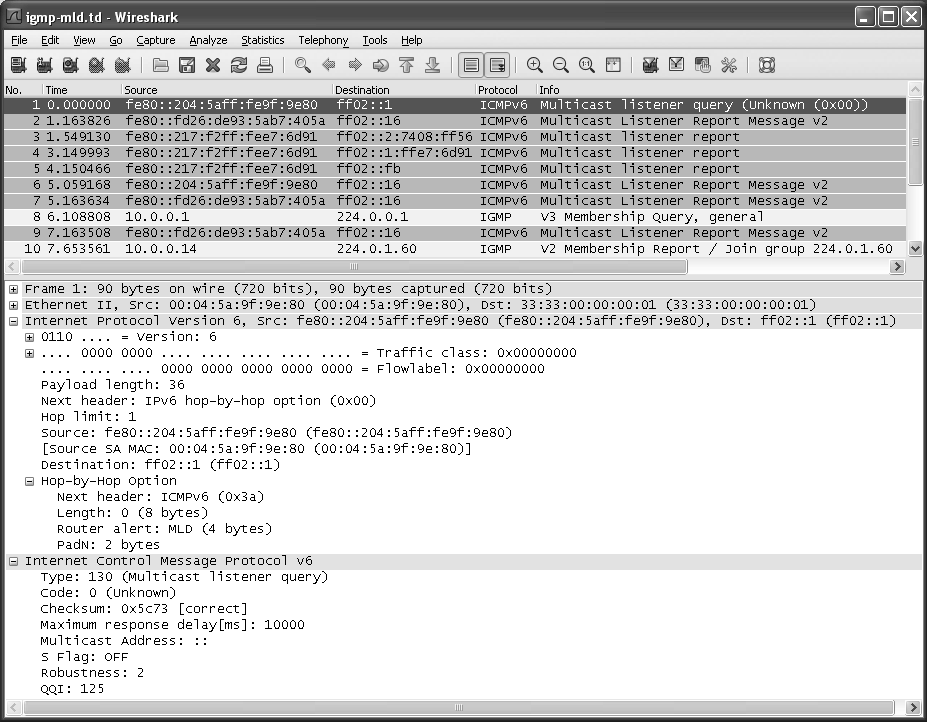
\includegraphics[width=1.0\textwidth]{imgs/9/9-12.png}
	\caption{1GMPv2、 IGMPv3、 MLDvl和MLDv2,全部在同一个子网。高亮的数据分组是一个MLD查询}
\end{figure}

\begin{figure}[ht]
    \centering
	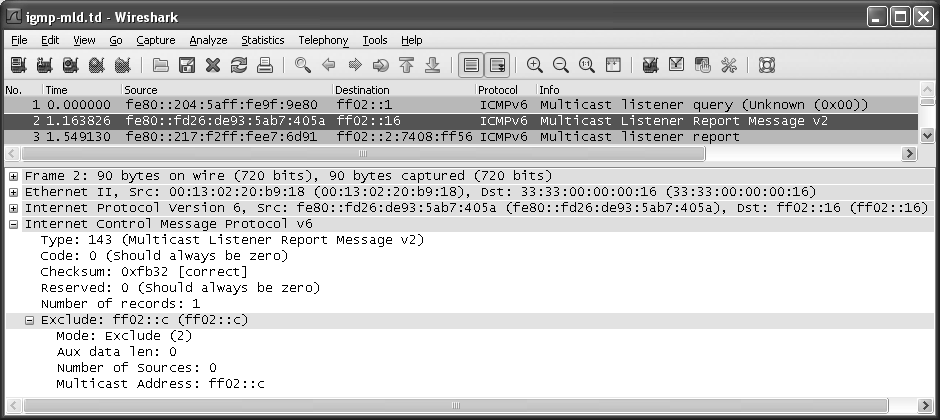
\includegraphics[width=1.0\textwidth]{imgs/9/9-13.png}
	\caption{通过使用没有源的排除类型的报文, MLDv2侦听报告报文表示了对组甜ff02::c的兴趣(SSDP本地链路范围组播地址)}
\end{figure}

图9-13是一个MLDv2 报告,表示对组播地址 ff02::c的兴趣(SSDP 的本地链路组找
址)。使用包含空源列表的排除模式报告,在这样的报告中指明了兴趣。跟踪记录中的随启
几个数据分组显示了 MLDv1 的使用(仍在一些系统中使用)。

图9-14中的分组3到分组5都是MLDvI 报告。只有分组3在这里显示,因其他白

分组是相似的(它们之间的区别仅在于各自的目的地IPv6地址不同)。与MLDv2 基本相同
每个报告都使用相同的结构,IPv6 基和扩展头部,但报告的目的地址是感兴趣的组播地均
ff02:2:7408:ff56。请注意,在MAC层,此目的地址映射到 33:33:74:08:ff:56。跟踪记录白
随后部分,从图9-15中的分组6开始,显示了MLDv2如何报告多个兴趣。
\begin{figure}[ht]
    \centering
	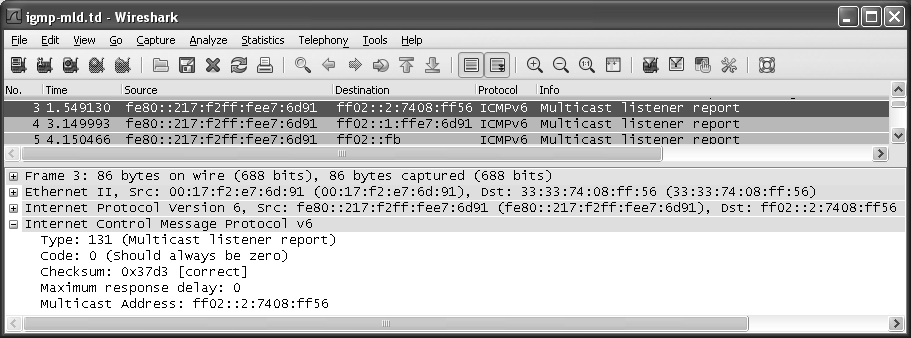
\includegraphics[width=1.0\textwidth]{imgs/9/9-14.png}
	\caption{MLDvl报告报文表示了对组播地址ffO2‥:2:7408:ff56的兴趣,该地址也是目的地IPv6地址}
\end{figure}

\begin{figure}[ht]
    \centering
	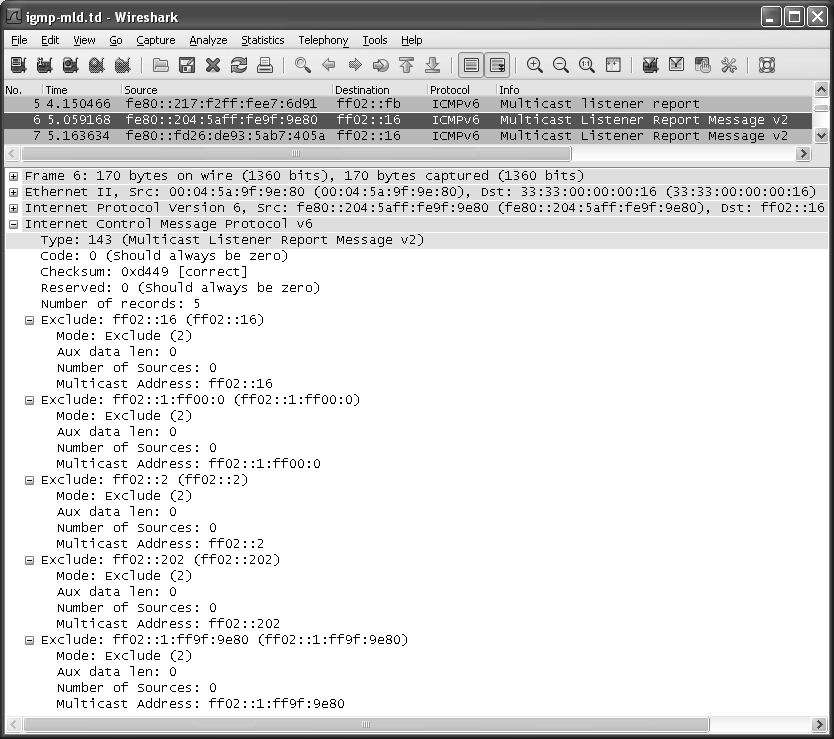
\includegraphics[width=1.0\textwidth]{imgs/9/9-15.png}
	\caption{MLDv2报告表达了对5个组播组的兴趣。每个组播地址记录通过指明没有源被排除,报告了对一个单一组的兴趣(即,模式为没有相关源的排除模式)}
\end{figure}

图9-15中的分组6是第一个 MLDv2报告,指明了对多个组播地址的兴趣。在这种情

况下,它来自 fe80:204:5aff:fe9f:9e80(MLD 查询方),并包含5个组的信息:f02:16(所
有具有MLDv2功能的路由器),ff02::1:f00:0(第一个请求节点地址),ff02::2(所有路由
器),f02:202(ONCRPC,一种远程过程调用),以及 ff02:1:f9f:9e80(其自身的请求节点
组)。分组7(不详细)是一个 MLDV2报告,指明主机 fe80:fd26:de93:5ab7:405a 对于它的请
求节点地址 ff02::1:ffb7:405a 感兴趣。我们现在转移到图9-16中显示的跟踪记录中的非 IPv6
流量。

图9-16中的分组8是记录的第一个 IPv4 分组,并且它是来自查询方10.0.0.1 的一个

IGMPv3的一般查询。该分组被发送到所有节点地址224.0.0.1,该组播地址映射到链路层地
址 01:00:5e:00:00:01。TTL 设置为1,因为IGMP报文不会通过路由器转发。IPv4 头部是24
个字节,比基本IPv4 头部多4个字节,这是为了保持4个字节的路由器警告选项。这个特
定的数据分组是一个IGMPv3成员查询,使用默认的最大响应时间10s、查询间隔125s。被
识别的组播地址(组) 0.0.0.0,所以这是请求了解所有使用中的组播组的一个一般查询。
分组9(未详细说明,但和分组7和2相似)是一个散布的MLDv2 响应,指明对组播地址
ff02::1:3(LLMNR)的兴趣。最后7个分组如图9-17所示。
\begin{figure}[ht]
    \centering
	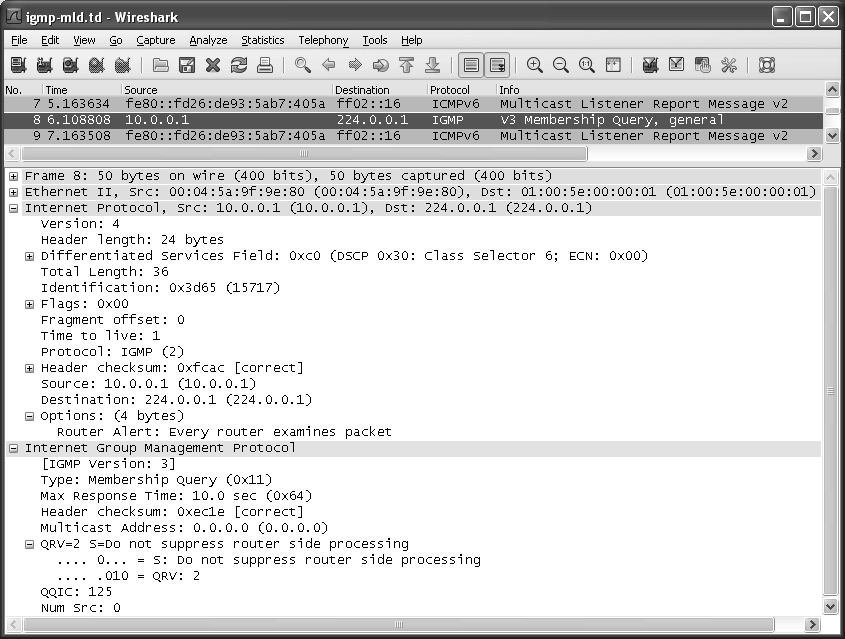
\includegraphics[width=1.0\textwidth]{imgs/9/9-16.png}
	\caption{一个IGMPv3一般成员资格查询,它被发送到所有节点组播地址 224.0.0.1。它的IPv4 头部包含一个值为0x30(类选择器6)的 DSCP 和IPv4 路由器警告选项}
\end{figure}

\begin{figure}[ht]
    \centering
	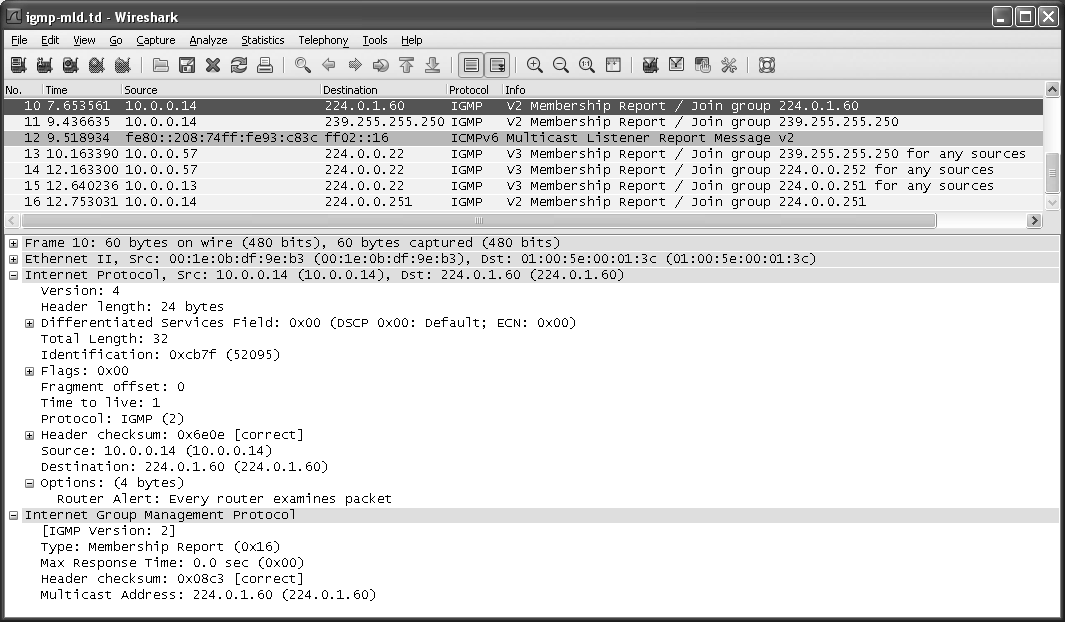
\includegraphics[width=1.0\textwidth]{imgs/9/9-17.png}
	\caption{分组10和最后7个分组的详细情况,它们是 IGMPv2 和 IGMPv3成员资格报告的混合(除丁分组12)。IGMPv2 的报告中不包含特定源的信息}
\end{figure}
在图9-17中的分组10是一个由10.0.0.14(连接到网络的打印机)发送到 224.0.1.60
的IGMPv2成员资格报告,它是一种发现服务,适用于惠普生产的设备。与MLDV1一样,
IGMPv2报文被发送到正在被引用的组的IP 地址。这样的报文 TTL =1,包括路由器警告选
项,长度为32个字节(24字节的IPv4 头部加上8字节的IGMP 报告信息)。


余下的数据分组没有详细列出,因为它们和我们已经详细看到的其他分组类似。分组
11报告,同一个系统 10.0.0.14希望加入组239.255.255.250(UPnP的一部分)。分组12是
一个MLDV2报告,说明主机 fe80::208:74ff:fe93:c83c 对组播地址 ff02:202(ONC RPC)和
ff02::1:f93:f83c(它的请求节点地址)感兴趣。分组13和分组14是IGMPv3报告,表明
IPv4地址为10.0.0.57的主机分别对组239.255.255.250 和 224.0.0.252 (LLMNR)感兴趣。最
后两个分组指明主机 10.0.0.13和 10.0.0.14希望加入组224.0.0.251(mDNS,见第11章)。
它们分别是 IGMPv3 和 IGMPv2报告。

\subsection{轻量级 IGMPV3 和 MLDv2}
正如我们已经看到的那样,主机维护对它们的应用和系统软件感兴趣的组播组的过滤器
状态。对于 IGMPv3或 MLDv2,它们也维护被排除或包含的源列表。为了了解什么流量需
要被转发到链路上以便有兴趣的主机收到,组播路由器维护类似的状态。反过来也是如此:
一个组播路由器可以停止转发在每个接收方的排除列表中的主机发送的组播流量。实践经验
证明,应用程序很少需要屏蔽特定源,并且支持此功能也比较复杂。然而,主机往往希望
包含一个与一个组相关联的特定源,尤其是当SSM 在使用时。因此,简化版的IGMPV3和
MLDv2已在\href{https://www.rfc-editor.org/rfc/rfc5790}{[RFC5790]}中定义,分别称为轻量级 IGMPv3(LW-IGMPv3)和轻量级 MLDV2
(LW-MLDv2)。

LW-IGMPv3 和LW-MLDv2是其正本的子集。它们支持ASM和SSM,并使用与
IGMPv3和 MLDv2 兼容的报文格式,但它们缺少特定阻塞源的功能。相反,唯一支持的排
除模式是没有列出源的情况,它对应于所有版本的IGMP或 MLD 中的传统的组加入(例如,
与图9-13中一样)。对于组播路由器,这意味着唯一需要的状态是记录哪些组感兴趣,以及
哪些源感兴趣。它不需要记录任何不期望的单个源。

表9-2显示了IGMPv3和 MLDv2 的轻量级变体中使用的报文类型的修改。在此表中,
空集符号(8)表示一个空的源地址列表。例如,TO\_EX({})表示一个0x04类型的报文,
说明它改变为没有相关源的EXCLUDE 模式。符号(*,G) 表示与任何源相关联的组G,符
号(S,G) 表示与特定源S相关联的组G。

表9-2

IGMPv3 和MLDv2的完整版本与它们的“轻量级”版本LW-IGMPv3 和 LW-MLDV2 的对比


比较表9-2与表9-1中的值。显而易见,没有使用非空排除模式,状态指示符类型已被
删除。此外,当前状态记录(IS\_EX 和IS\_EN)已对兼容的主机删除。轻量级组播路由器仍
然应该能够接收这样的报文,但对待它们就好像它们总是包含一个空源列表。

\subsection{IGMP 和 MLD 健壮性}
对于IGMP 和MLD 协议的健壮性和可靠性有两个主要的问题。IGMP或 MLD 的失效,

或更一般的组播,可以导致不需要的组播流量的分配,或没有能力交付期望的组播流量。由
IGMP 和 MLD 处理的失败类型包含组播路由器的失效和协议报文的丢失。

通过允许多个组播路由器在同一链路上运行,可以处理组播路由器潜在的失效故障。正

如前面提到的,在这样的配置中,具有最小P 地址的路由器被选“查询器”。查询器负责
发送一般和特定查询来确定该子网中主机的当前状态。其他(非查询器)路由器监控协议报
文,因为它们也是组成员或组播混杂侦听器,并且假如当前查询器失效了,不同的路由器能
够作为查询器介人。为了使其正常工作,所有连接到相同链路的组播路由器需要协调它们的
查询、响应和它们的一些配置信息(主要是计时器)。

多个组播路由器实现的第一种类型的协调是查询器选举(querier election)。每个组播路

由器可以侦听其他的查询。当一个组播路由器启动时,它认为自己是查询器,并发送一般查
询以确定在子网中哪些组是活跃的。当一个路由器收到另一个路由器的组播查询时,它比较
源IP地址和它自己的。如果在所接收的查询中的源IP 地址小于它自己的,接收路由器进入
备用模式。因此,具有最小IP地址的路由器被认为是获胜者,并成为单一的查询器,负责
向它连接的子网中发送查询。备用的路由器设置计时器,如果它们在一个指定的时间(称为
其他查询器出现(other-querier-present)计时器)内没有看到更多的查询,它们再次成为查
询器。

查询组播路由器定期发送一般查询,以确定哪些组和主机是同一个子网的主机感兴趣

的。这些查询被发送的频率由查询器的查询间隔、可配置计时器参数决定。当多个组播路由
器在同一子网中运行时,当前查询器的时间间隔被所有其他路由器接受。在这种方式中,如
果当前查询器失效,到替代组播路由器的切换不会干扰定期查询速率。

有理由相信,一个组(或源)不再感兴趣的组播路由器发送一个特定的优先查询以停止

相应组播流量的转发(或通知组播路由协议)。这些查询以不同于一般查询的时间间隔(称
最后成员查询时间(Last Member Query Time,LMQT)发送。LMQT 通常比查询间隔要小
(短),并管理离开延迟。当多个组播路由器在同一个子网运行时,可能同时出现一个问题,
主机希望离开组(或丢弃源),并且协议信息会丢失。

为了帮助防止丢失协议报文,有些报文被重传多次(由QRV 查询器鲁棒性变量决定)。

QRV 值在包含于查询中的QRV 字段中编码,非查询路由器采用查询器的QRV 作为自己的。
如果查询器发生改变,这再次帮助保持了稳定性。重传中保护的报文类型包括状态改变报告
和特定查询。其他报文(当前状态报告)通常不会导致转发状态的变化,而是只涉及通过调
整计时器刷新软状态,所以使用重传无法保护它们。当重传发生时,报告的重传间隔在0和
一个称为主动报告间隔(Unsolicited Report Interval)的可配置参数之间随机选择,查询的重
传间隔是周期性的(基于LMQT的间隔)。预计更容易出现丢失的链路(如无线链路),可能
需要以生成额外的流量为代价,增加鲁棒性变量以增强分组丢失的健壮性。

当处理特定查询时,为了帮助组播路由器保持同步,查询报文中S位字段表明路由器

端(计时器)处理应被抑制。当一个特定的查询由查询器发送时,应该安排一个重传次数
(QRV)。在发送的第一个查询中,S位字段被清除。基于重传或这种查询的接收,组播路由
器会为随后的重传降低它的计时器到LMQT。此时,为感兴趣的主机提供一个报告,指出它
对一个组或源的持续的兴趣,这是可能的。如果没有报文丢失,该报告使每个组播路由器重
置它的计时器为普通值,并保持不变。然而,预定的重传不会被放弃。相反,特定查询的重
传被发送时,S位字段被设置,这将导致接收路由器不会降低它们的计时器到 LMQT。

在收到表示有兴趣的报告之后,仍保持查询重传的原因,是为了使跨越所有组播路由器

的组的超时时间是一致的。然后,S位字段的目的是为了让特定的查询被(重新)发送,也
为了避免降低计时器到LMQT,因为一个表示兴趣的合法的报告可能已经被接受了,即使它
或初始查询被非查询器路由器丢失了。没有这种能力,重传的特定查询会导致非查询器路

器不正确地降低它们的计时器(因为已经收到一个表明兴趣的合法报告)。

\subsection{IGMP 和MLD 计数器和变量}
IGMP 和 MLD是软状态的协议,它们也处理路由器的失效、协议报文的丢失以及与早

期协议版本的互操作性。很多设备是基于触发状态改变和协议动作的计时器来启用这些功能
的。表9-3总结了IGMP 和 MLD 使用的所有的配置参数和状态变量。

在表9-3中,很显然,MLD 和IGMP 共享大部分的计时器和配置参数,虽然在某些情

况下术语是不同的。那些表示为“不能改变”的一些值是根据其他值设置的,不能独立变化。
表9-3 IGMP和 MLD 的参数和计时器的值。大多数值可以作为配置参数在一些实现中改变

名称和意义

默认值(限制)

鲁棒性变量(Robustness Variable,RV)——为一些状态改变报告/查询安排

2(不能为0;不应该为1)

多达 RV-1次的重传

查询间隔(Query Interval,QI)—当前查询器发送的一般查询之间的时间

125s

查询响应间隔(Query Response Interval,QRI) —等待产生报告的最大响

10s

应时间。该值编码形成最大响应字段

广播和本地组播(IGMP和MLD)

331

(续)

名称和意义

IGMP 中的组成员间隔(Group Membership Interval, GMI) 和 MLD 中的组

播地址侦听间隔(Multicast Address Listening Interval, MALI)—对于组播

路由器来说,没有看到一个报告所必须经过的时间,用以宣布对于一个组或是

源/组的组合没有兴趣了

IGMP 中的其他查询出现间隔 (Other Querier Present Interval) 和 MLD 中的

其他查询出现超时(Other Querier Present Timeout)—对于一个非查询器组

播路由器来说,没有看到一个一般查询所必须经过的时间,用以宣布没有活动

的查询器

启动查询间隔(Startup Query Interval)

-查询器刚启动时发送的一般查询

之间的时间间隔

启动查询数量(Startup Query Count).

-查询器刚启动时发送的一般查询

的数量

IGMP 中的最后成员查询间隔(Last Member Query Interval, LMQI)和

MLD 中的最后侦听方查询间隔(Last Listener Query Interval,L.LQI)—等

待响应特定查询的报告产生的最大响应时间。该值编码形成特定查询中的最大

响应字段

IGMP 中的最后成员查询数量(Last Member Query Count) 和 MLD 中的最

后侦听方查询数量(Last Listener Query Count)——发送特定查询而没有接收

到响应的数量,用以宣布没有感兴趣的主机

主动报告间隔(Unsolicited Report Interval)—

一主机初始状态改变报告重传

之间的时间

旧版本查询器出现超时(Older Version Querier Present Timeout)

一主机没

有接收到 IGMPvI或IGMPv2请求报告而恢复到IGMPv3所需要等待的时间

IGMP 中的旧主机出现间隔 (Older Host Present Interval) 和 MLD 中旧版本

主机出现超时 (Older Version Host Present Timeout)

一查询器没有接收到

IGMPv1或IGMPv2 报告报文而恢复到IGMPv3所需要等待的时间

默认值(限制)

RV *QI + QRI(不能改变)

RV *Q1+(0.5)*QRI(不能改变)

(0.25)* Q1

RV

1s

RV

RV *QI+ QRI(不能改变)

RV *Q1 +QRI(不能改变)

\subsection{IGMP 和MLD探听}
IGMP 和MLD管理路由器之间IP 组播流量的流动。为了进一步优化流量流动,对于第

2层交换机(即通常不会处理第3层IGMP或 MLD 报文)来说,通过查看在第3层的信息了
解它对特定的组播流量流动是否有兴趣,这是可能的。该功能通过称为 IGMP(MLD)採听
(snooping)\href{https://www.rfc-editor.org/rfc/rfc4541}{[RFC4541]}的交换机特征指明,并且被很多交换机供应商支持。没有IGMP探听,
交换机通常沿着所有交换机形成的生成树的所有分支广播它来发送链路层流量。这是一种浪
费,如我们前面描述的原因。IGMP(MLD)感知的(有时也把IGMP 探听称为IGS)交换机
监控主机和组播路由器之间的IGMP(MLD)流量,并且能记录哪些端口需要哪些特定的组
播流动,这和组播路由器的做法很相似。这样做能够实质地影响在一个交换网络中正在被承
载的不需要的组播流量的数量。

有几个细节使得IGMP/MLD 探听的直接实现变得复杂。在IGMPv3和 MLDv2中,生

成报告响应查询。然而,在这些协议的早期版本中,一台主机生成的报告,被相同链路上的
其他组成员侦听,导致了其他成员抑制它们的报告。如果IGS 交换机要将报告转发到所有连
接的接口上,这可能会导致一个问题,因为在一些LAN(VLAN)段上的主机和组成员可能
没有被通知。因此,支持早期版本的IGMP 和 MLD 的IGS交换机避免向所有的接口广播报
告。相反,它们只向最近的组播路由器转发报告。如果使用组播路由器发现(MRD)(见第8
章),确定组播路由器的位置就变得更简单了。

实现探听时的另一个值得关注的问题是IGMP和 MLD之间的报文格式上的差异。由于

MLD 被封装为ICMPv6的一部分,而不是自己单独的协议,因此MLD 探听交换机必须处理
ICMPv6信息,并小心地从其他报文中分离出 MLD 报文。尤其是,由于ICMPv6用于其他
各种功能(见第8章),其他的ICMPv6流量必须被允许自由流动。

其他非标准的专有协议已经被实现,可以进一步优化通过第2层设备运载的IP组播

流量。例如,思科提出了路由器端口组管理协议(Router-port Group Management Protocol,
RGMP) \href{https://www.rfc-editor.org/rfc/rfc3488}{[RFC3488]}。在RGMP 中采用了一种机制,这样主机不仅报告它们的组和感兴趣的
源(如在IGMP/MLD 中),而且组播路由器也这样做。该信息用来优化组播路由器(不仅仅
是主机)之间的组播流量在第2层的转发。

\section{与IGMP和MLD相关的攻击}

由于IGMP 和 MLD是信令协议,可以控制组播流量的流动,使用这些协议的攻击主要
是DoS攻击或资源使用攻击。也有攻击利用协议的实现错误来禁用主机或导致它们执行攻击
者提供的代码。

一个简单的DoS攻击可以通过发送IGMP 或MLD来订阅大量的高带宽的组播组来发
起。这样做会引起带宽耗尽,导致拒绝服务。一个更复杂的攻击可能通过使用相对较小的IP
地址生成请求来发起。在这种情况下,攻击者当选链路的查询器,可以通知它自己的鲁棒
性变量、查询时间间隔和将要被其他组播路由器采用的最大响应时间。如果最大响应时间是
非常小的,主机被诱导来迅速发送报告,消耗了 CPU 资源。

一些攻击已经通过利用实现错误来实施。分片的IGMP 分组已经被用来在特定的操作系

统中诱导崩溃。最近,使用SSM 信息的特制的IGMP 或MLD报文已经用于诱导远程代码执
行错误。总体而言,IGMP或MLD 漏洞的影响往往比其他协议要小,因为组播往往只是支
持当地。其结果是,缺乏接入到目标LAN的链路的远程攻击者可能是有限的。

\section{总结}

一般来说,广播是指向网络上的所有节点发送流量。在TCP/IP 的背景下,广播是指向
网络或子网中的所有主机发送一个数据分组,通常是本地连接的网络。组播是只向网络中的
一个子集节点发送流量。在TCP/P 中,组播是指向网络中感兴趣的主机的一个子集发送数
据分组。选择子集的方法依赖于组播流量的范围和接收方的兴趣。在许多应用中,组播比广
播更好,因为组播给没有参加通信的主机带来更少的开销。广播在IPv4 中支持,但在IPv6
中不支持。广播和组播可以避免通过重复使用单播连接将相同的内容发送到多个目的地。它
也可以被用于发现未知的服务器。组播是比广播更复杂的一种功能,因为必须维护状态以确
定哪些主机对哪些组有兴趣。

在IPv4 中,有两种类型的广播地址:受限(255.255.255.255)和定向。定向广播地址
基于网络前缀和它的长度,通过创建一个初始位和网络前缀相等、低序位被置1 的32位地
址形成。通常使用定向广播代替受限广播地址是更可选的。选择哪些接口用于发送传出的广
播流量依赖于操作系统。一个典型的例子是使用一个主接口用于有限广播流量,使用保存在
主机的转发表中的信息来选择传出定向广播和组播的接口。

IP 的组播支持一种模型,借以实现对接收组播数据分组感兴趣的进程在一组特定接口上
订阅一个特定组(使用IP地址)。在具有组播功能的IEEE 链路层网络上(如以太网),传输
组播IPv4流量涉及结合组地址的低序23位和前缀01:00:5e 来形成用于链路层组播的MAC
层目的地址。传输 IPv6组播流量涉及结合组地址的低序32位和16位前缀33:33来形成
MAC层目的地址。这些映射不是唯一的,也就是说,多个IPv4或IPv6 组地址使用相同的
MAC层地址。因此,主机软件执行传入流量过滤以除去不需要的组流量。

IGMP 和 MLD 协议分别在IPv4 和 IPv6 中用于支持组播数据分组交付。组播路由器向
附近的主机发送查询报文以确定哪些主机对哪些组有兴趣,以及(对于 IGMPv3和 MLDV2)
哪些发送者对这些组来说是感兴趣的。主机通过发送报告来响应,该报告指明了对组的
兴趣。MLD是ICMPv6协议的一部分,而IGMP是一个位于IPv4上层的独立协议(例如
ICMP)。有些交换机配备了“探听”IGMP 和 MLD 流量的功能,用以避免沿着生成树分支
发送组播IP 流量,因为其中有些分支存在没有兴趣的接收主机。IGMP 和 MLD 有一个“鲁
棒性变量”,可以设置来启用网络上易于丢失的重要信息的重传。

由于IGMP 和 MLD 都是信令协议,可以控制其他流量的流动,针对它们的攻击往往会
引起额外的资源消耗,可能导致拒绝服务。其他形式攻击利用已经发现的实现漏洞,导致执
行由攻击者提供的不需要的代码。由于 MLD(和 MLDv2)在部署方面相对较新,发现额外
的漏洞是有可能的,但这些协议限制在单一链路的操作。

\section{参考文献}
[CK11] S. Cheshire and M. Krochmal, "Multicast DNS," Internet draft-cheshire-

dnsext-multicastdns, work in progress, Feb.2011.

[EGW02]B. Edwards, L. Giuliano, and B. Wright, Interdomain Multicast Routing:

Practical Junper Networks and Cisco Systems Solutions (Addison-Wesley, 2002).

IGCLG99] Y.Goland, T. Cai, P. Leach, and Y. Gu, "Simple Service Discovery

Protocol/1.0 Operating without an Arbiter" Internet draft-cai-ssdp-V1-03.txt

(expired), Oct. 1999.